% Презентация ЛР2 (вариант 4-4-2: матрица Фишера · вынос за 3σ · KL). Сборка: python scripts/build_slides.py
% (пишет numbers.tex и fonts.tex, проверяет рисунки, компилирует tectonic -X compile lab2_presentation.tex).
% Рисунки — figures/, их делает lab02_criteria.ipynb (lab02/report.py); числа — numbers.tex из results/.
\documentclass[11pt,aspectratio=43]{beamer}
\usepackage{iftex}
\ifXeTeX
  \usepackage{fontspec}
  \input{fonts.tex}
  \usepackage{polyglossia}
  \setmainlanguage{russian}
\else
  \usepackage[T2A]{fontenc}
  \usepackage[utf8]{inputenc}
  \usepackage[russian]{babel}
\fi
\usepackage{amsmath,amssymb}
\usepackage{booktabs}
\usepackage{array}
\usepackage{graphicx}
\graphicspath{{../figures/}}
% Written by scripts/build_slides.py from results/; do not edit.
\newcommand{\Threshold}{1.92}
\newcommand{\Zeff}{2.13}
\newcommand{\MCcount}{16}
\newcommand{\MCFisherD}{2/16}
\newcommand{\MCGodambeD}{1/16}
\newcommand{\MCFisherDExpected}{2.4}
\newcommand{\MCGodambeDExpected}{0.3}
\newcommand{\MCFisherUnderMin}{2}
\newcommand{\MCFisherUnderMax}{4}
\newcommand{\MCGodambeUnderA}{1.9}
\newcommand{\NarrowSynMin}{1.9}
\newcommand{\NarrowSynMax}{2.2}
\newcommand{\NarrowRealMin}{1.6}
\newcommand{\NarrowRealMax}{1.8}
\newcommand{\SynAKLD}{\ensuremath{0.52}}
\newcommand{\SynBThetaD}{\ensuremath{0.0083 \pm 0.0015}}
\newcommand{\SynBKLD}{\ensuremath{12.5}}
\newcommand{\SynBQstarD}{0.6\,\%}
\newcommand{\RealWindows}{4802}
\newcommand{\RealQstar}{\ensuremath{3.1\cdot10^{-4}}}
\newcommand{\RealQstarWindows}{2}
\newcommand{\HuberRatio}{5}
\newcommand{\PlaceboRatio}{98}
\newcommand{\HuberShiftA}{1.1}
\newcommand{\VinSigma}{0.16}
\newcommand{\OrdersAV}{3.8}
\newcommand{\GridSigmaReal}{0.05}
\newcommand{\LeafLossMin}{4}
\newcommand{\LeafLossMax}{5000}
\newcommand{\LeafKL}{0.19}
\newcommand{\WindowKL}{\ensuremath{1.1\cdot10^{3}}}
\newcommand{\ThetaAmin}{0.72}
\newcommand{\ThetaAmax}{0.85}
\newcommand{\StepKLV}{0.39}
\newcommand{\RsqFull}{0.4021}
\newcommand{\RsqFinal}{0.4019}
\newcommand{\GraphBeforeText}{20 вершин, 19 рёбер}
\newcommand{\GraphAfterRealText}{9 вершин, 8 рёбер}
\newcommand{\NTests}{79}
\newcommand{\RealThetaA}{\ensuremath{0.794 \pm 0.013}}
\newcommand{\RealQA}{\ensuremath{0.0574 \pm 0.0020}}
\newcommand{\RealKLA}{\ensuremath{1.5\cdot10^{3}}}
\newcommand{\RealShapeA}{\ensuremath{1.41}}
\newcommand{\RealThetaV}{\ensuremath{-4.4 \pm 6.4}}
\newcommand{\RealQV}{\ensuremath{0.03 \pm 0.49}}
\newcommand{\RealKLV}{\ensuremath{0.23}}
\newcommand{\RealShapeV}{\ensuremath{2.09}}
\newcommand{\RealThetaD}{\ensuremath{-0.19 \pm 0.90}}
\newcommand{\RealQD}{\ensuremath{-0.018 \pm 0.066}}
\newcommand{\RealKLD}{\ensuremath{0.018}}
\newcommand{\RealShapeD}{\ensuremath{2.13}}
\newcommand{\DecisionRows}{    синтетика А & \textcolor{keep}{оставить} & \textcolor{keep}{оставить} & \textcolor{drop}{удалить} & 14 / 13 \\
    синтетика Б & \textcolor{keep}{оставить} & \textcolor{keep}{оставить} & \textcolor{keep}{оставить} & 18 / 17 \\
    эксперимент & \textcolor{keep}{оставить} & \textcolor{drop}{удалить} & \textcolor{drop}{удалить} & 9 / 8 \\}


% ---------- оформление в стиле образца ----------
\definecolor{mred}{RGB}{200,16,46}
\definecolor{mgray}{RGB}{236,236,236}
\setbeamertemplate{navigation symbols}{}
\setbeamercolor{frametitle}{fg=mred,bg=mgray}
\setbeamercolor{title}{fg=mred,bg=mgray}
\setbeamercolor{structure}{fg=mred!80!black}
\setbeamercolor{block title}{fg=black}
\setbeamerfont{frametitle}{size=\large}
\setbeamertemplate{frametitle}{%
  \nointerlineskip
  \begin{beamercolorbox}[wd=\paperwidth,ht=3ex,dp=1.4ex,leftskip=0.6em]{frametitle}%
    \usebeamerfont{frametitle}\insertframetitle
  \end{beamercolorbox}}
\setbeamertemplate{footline}{%
  \hfill\usebeamerfont{footline}\scriptsize\insertframenumber\,/\,\inserttotalframenumber\hspace{1em}\vspace{0.8ex}}
\setbeamertemplate{itemize items}[circle]
\setbeamertemplate{enumerate items}[default]
\setbeamersize{text margin left=1.2em,text margin right=1.2em}
\newcommand{\head}[1]{\textbf{#1}\par}
\newcommand{\src}[1]{{\scriptsize\color{black!60}#1}}
\definecolor{keep}{RGB}{0,131,0}
\definecolor{drop}{RGB}{227,73,72}
\newcommand{\KL}{\mathrm{KL}}
\newcommand{\KLs}{\mathrm{KL}_{\text{сдв}}}

\title{Интервенции и выбор элементов графа:\\ уравнение Навье–Стокса для следа ветротурбины}
\subtitle{Лабораторная работа 2 · вариант 4-4-2}
\author{Карпеев Глеб}
\date{2026}

\begin{document}

% ---------- титульный ----------
\begin{frame}[plain]
  \vspace*{-0.4em}
  \begin{beamercolorbox}[wd=\textwidth,sep=0.9em,center]{title}
    {\large\inserttitle}\par\vspace{0.4em}
    {\color{black}\normalsize\insertsubtitle}
  \end{beamercolorbox}
  \vspace{2.2em}
  \centering
  \insertauthor\par\vspace{2.5em}
  \insertdate
\end{frame}

% ---------- постановка ----------
\begin{frame}{Задание}
  \head{Цель}
  Выработать критерий удаления вершин и рёбер графа модели из ЛР~1: провести интервенцию над данными,
  сравнить распределения параметров до и после и принять решение.
  \bigskip

  \head{Тройка методов}
  \small
  \begin{tabular}{@{}lc>{\raggedright\arraybackslash}p{0.5\textwidth}@{}}
    \toprule
    & пункт & метод \\
    \midrule
    оценка распределения & 1.4 & матрица Фишера вектора и подвектора \\
    интервенция & 2.4 & вынос за три сигмы с учётом условного распределения \\
    расстояние & 3.2 & Кульбака–Лейблера \\
    \bottomrule
  \end{tabular}
  \bigskip

  \head{Модель и данные}
  Модель ЛР~1 чужая: уравнение импульса Навье–Стокса А.~Эйнуллаева [2].
  Синтетика DNS с известным ответом (два сценария); эксперимент — объёмные поля скорости VIC\#
  в следе модели ветротурбины [1].
\end{frame}

\begin{frame}{1. Уравнение из ЛР 1}
  Правая часть уравнения импульса — дерево выражения из 16 вершин и 15 рёбер:
  \[
    \partial_t u=-(\nabla u)\,u-\nabla p/\rho+\nu\,\Delta u .
  \]
  Решение принимаем о ветвях итоговой суммы — у каждой свой параметр:
  \[
    \partial_t u=\theta_A\bigl[-(\nabla u)u\bigr]-\theta_P\,\nabla p+\theta_V\,\nu_{\text{ЛР1}}\Delta u+\theta_D\,(-u),
  \]
  в ЛР~1 $\theta_A=\theta_V=1$, $\theta_P=1/\rho$, $\theta_D=0$.
  \bigskip

  \begin{itemize}
    \item Удалить элемент $\Leftrightarrow$ $\theta_e=0$.
    \item $D=-\alpha u$ (трение) в ЛР~1 нет: это контроль. Критерий должен удалить его, когда трения нет,
      и оставить, когда есть.
  \end{itemize}
\end{frame}

\begin{frame}{2. Параметры и элементы графа}
  \centering
  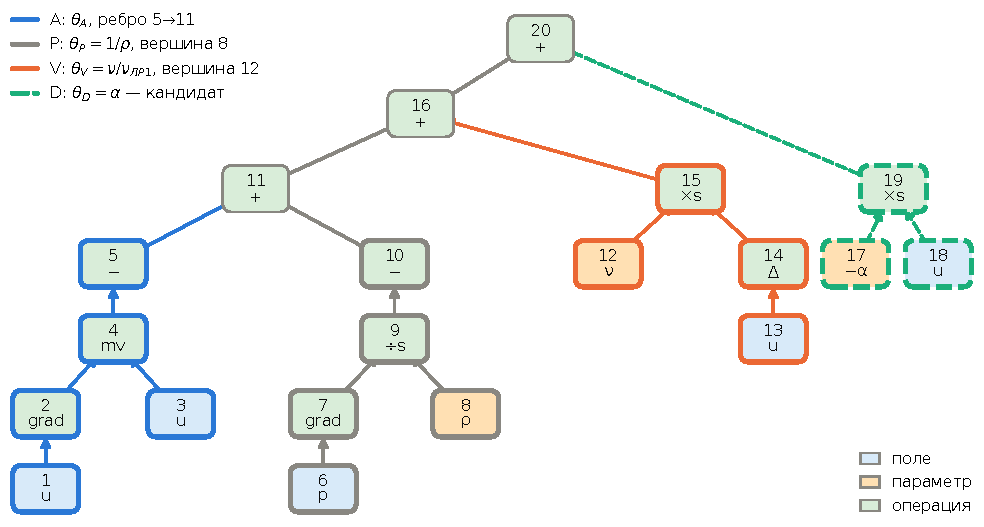
\includegraphics[width=\textwidth,height=0.62\textheight,keepaspectratio]{tree}
  \par\medskip\raggedright\small
  Рамка вершины — элемент: $A$ — вес ребра 5$\to$11, $P$ — $\theta_P=1/\rho$ (вершина 8),
  $V$ — $\nu$ (вершина 12), $D$ — кандидат $-\alpha u$ (вершины 17–19).
  Кандидатный граф: \GraphBeforeText.
\end{frame}

\begin{frame}{2. Что можно оценить по данным}
  \begin{columns}[T]
    \begin{column}{0.56\textwidth}
      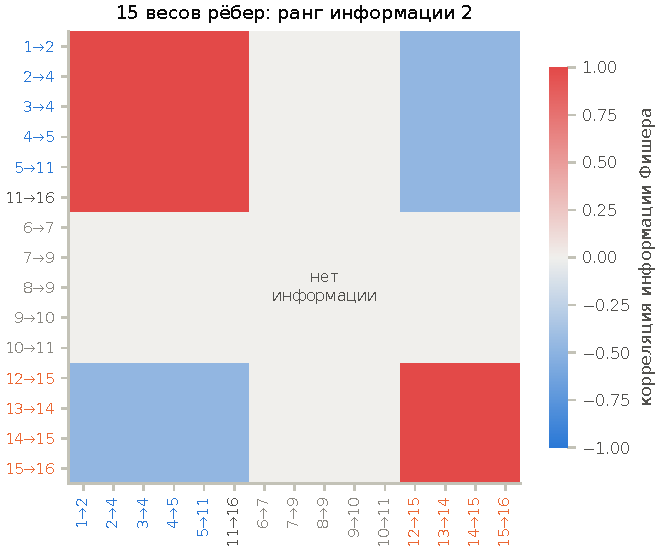
\includegraphics[width=\linewidth]{identifiability}
    \end{column}
    \begin{column}{0.43\textwidth}
      \scriptsize
      \head{Слабая форма [15]}
      Уравнение интегрируется с гладкой пробной функцией по окну: $y=X\theta+r$, строка — окно,
      столбец — значение ветви.
      \smallskip

      \head{Давление}
      Пробные функции соленоидальны $\Rightarrow$ столбец давления $\equiv0$: $p$ и $\rho$ по скорости
      не определяются, $\rho$ сливается в $P=p/\rho$.
      \smallskip

      \head{Подвектор}
      Информация 15 весов рёбер имеет ранг 2: внутри ветви рёбра неразличимы $\Rightarrow$ оцениваем
      $\theta=(\theta_A,\theta_V,\theta_D)$.
    \end{column}
  \end{columns}
\end{frame}

% ---------- метод ----------
\begin{frame}{3. Метод: матрица Фишера (1.4)}
  \small
  \head{Распределение}
  Приближение Лапласа $\theta\sim\mathcal N(\hat\theta,F^{-1})$, $F=X^\top X/\sigma^2$ [3, 4];
  подвектор — блок $F^{-1}$ (информация за вычетом объяснённой другими параметрами).
  \smallskip

  \head{Зависимые строки}
  Окна перекрываются $\Rightarrow$ информация Годамбе $G=HJ^{-1}H$, $J$ — ковариация градиента $S$,
  суммированного по кластерам соседних окон [5, 6].
  \smallskip

  \head{Функции ошибки}
  L2 и Хьюбер ($c=1.345$): квадратичная около нуля, линейная в хвостах [7].
  \smallskip

  \head{Почему подходит}
  Модель линейна по параметрам элементов $\Rightarrow$ гауссово приближение точное при тысячах окон,
  распределение в замкнутом виде, без шума сэмплирования.
  \smallskip

  \head{Проверки, не метод}
  Форма — кластерный бутстрэп (это п.~1.1, решения по нему не принимаются); ширина — \MCcount{} независимых
  реализаций DNS. Решения — по L2 + Годамбе.
\end{frame}

\begin{frame}{3. Метод: вынос за три сигмы (2.4)}
  \small
  Переменная — вход элемента $e$ в окне $x_e$; условный закон $x_e\mid x_{-e}\sim\mathcal N(\mu,\sigma^2)$,
  $\mu$ — регрессия на входы других элементов. В доле $q$ окон:
  \[
    x_e'=\mu+\operatorname{sign}(x_e-\mu)\,k\sigma,\qquad k\ge3 .
  \]
  \vspace{-0.6em}
  \centering
  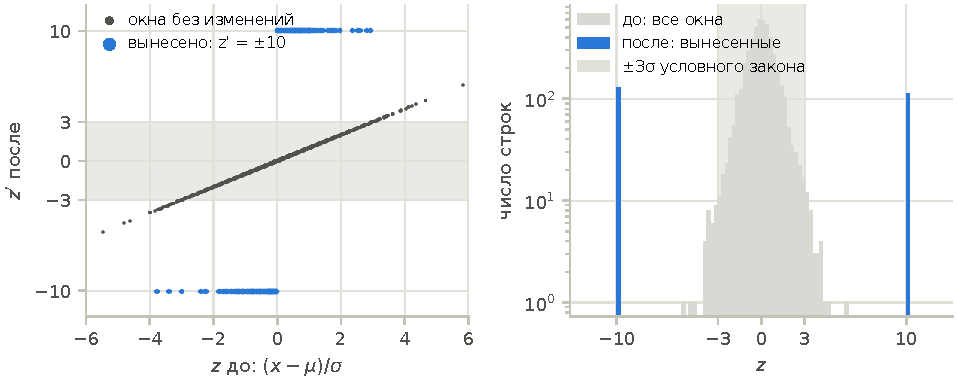
\includegraphics[width=0.92\textwidth,height=0.4\textheight,keepaspectratio]{intervention}
  \par\raggedright\footnotesize
  Условный: по теореме Фриша–Во–Ловелла $\theta_e$ определяется только остатком $x_e-\mu$ — его и разрушаем [11].
  В $\pm3\sigma$ лежит $\ge95\,\%$ массы унимодального закона [8] $\Rightarrow$ вынесенное — выбросы.
  Потеря параметра: $\rho(k,q)=1-\dfrac{1-q+qk\sqrt{2/\pi}}{1-q+qk^2}$.
\end{frame}

\begin{frame}{3. Метод: расстояние Кульбака–Лейблера (3.2)}
  \small
  $P$ — распределение до интервенции, $Q$ — после [12]:
  \[
    \KL(Q\|P)=\underbrace{\tfrac12(m_Q-m_P)^\top\Sigma_P^{-1}(m_Q-m_P)}_{\text{сдвиг}}
    +\underbrace{\tfrac12\bigl[\operatorname{tr}(\Sigma_P^{-1}\Sigma_Q)-d-\ln\det\Sigma_P^{-1}\Sigma_Q\bigr]}_{\text{форма}}
  \]
  \begin{itemize}
    \item $\KL\approx\tfrac12\delta^\top F\delta$: матрица Фишера — метрика KL [13] $\Rightarrow$ одна геометрия с 1.4.
    \item Полностью разрушенная информация: сдвиг $=S_e=\hat\theta_e^2/2\sigma_e^2$ — KL до ближайшей
      модели без элемента [14]; при силе $(k,q)$: $\KLs\approx\rho(k,q)^2S_e$.
    \item Форма растёт и у несуществующих элементов (дисперсия входа меняется в $k^2$ раз)
      $\Rightarrow$ в решение входит только сдвиг.
  \end{itemize}
\end{frame}

\begin{frame}{3. Правило и совместимость тройки}
  \small
  \head{Правило}
  Вход $e$ выносится за $k=10$ сигм во всех окнах ($q=1$):
  \[
    \text{оставить } e\iff\KLs(Q_e\|P_e)>\tfrac12\chi^2_1(0.95)=\Threshold\ \text{нат}\ \text{и знак }\hat\theta_e\text{ допустим}.
  \]
  Знаки: $\theta_A,\nu,\alpha>0$. Эквивалентно $|\hat\theta_e/\sigma_e|>1.96/\rho=\Zeff$ — тест Вальда.
  Удаляем по одному (слабейший) и переоцениваем.
  \medskip

  \head{Совместимость}
  \begin{itemize}
    \item 1.4 даёт распределение и метрику $F$, 2.4 сдвигает распределение, 3.2 меряет сдвиг в метрике $F$ —
      всё в замкнутых формулах.
    \item Условная $\sigma$ интервенции — та же остаточная дисперсия входа, из которой оценён блок подвектора.
    \item $q^*$ — доля испорченных окон, при которой элемент становится «заметен».
  \end{itemize}
\end{frame}

\begin{frame}{4. Вычислительный эксперимент}
  \small
  \begin{enumerate}
    \setlength{\itemsep}{0pt}
    \item Слабая форма $\Rightarrow$ $y$, $X$ (столбцы — ветви $A$, $V$, $D$).
    \item $\hat\theta$ и 4 распределения: (L2, Хьюбер) $\times$ (Фишер, Годамбе) $\Rightarrow$ $P$.
    \item Вынос входа каждого элемента: $k\in[3;30]$ при $q=5\,\%$, $q\in[10^{-4};1]$ при $k=10$, 10 сидов $\Rightarrow$ $Q$.
    \item $\KL(Q\|P)$: сдвиг и форма; решение при $k=10$, $q=1$; обратное исключение.
    \item Проверки: \MCcount{} реализаций DNS, бутстрэп, плацебо, вынос на сетке, 5 размеров окон.
  \end{enumerate}
  \smallskip
  {\footnotesize
  \begin{tabular}{@{}lll@{}}
    \toprule
    данные & что & истина \\
    \midrule
    синтетика А & DNS Навье–Стокса $48^3$, шум 5\,\% & $\theta_A=\theta_V=1$, $\theta_D=0$ \\
    синтетика Б & то же $+$ трение $-\alpha u$ & $\theta_D=\alpha=0.01$ \\
    эксперимент & VIC\#, 86 кадров 500 Гц, $53\times33\times33$ & неизвестна \\
    \bottomrule
  \end{tabular}}
  \smallskip

  Код — пакет \texttt{lab02/}, отделён от ноутбука; код ЛР~1 подключён без изменений; \NTests{} тестов.
\end{frame}

% ---------- синтетика ----------
\begin{frame}{5. Синтетика А: распределения по методам}
  \centering
  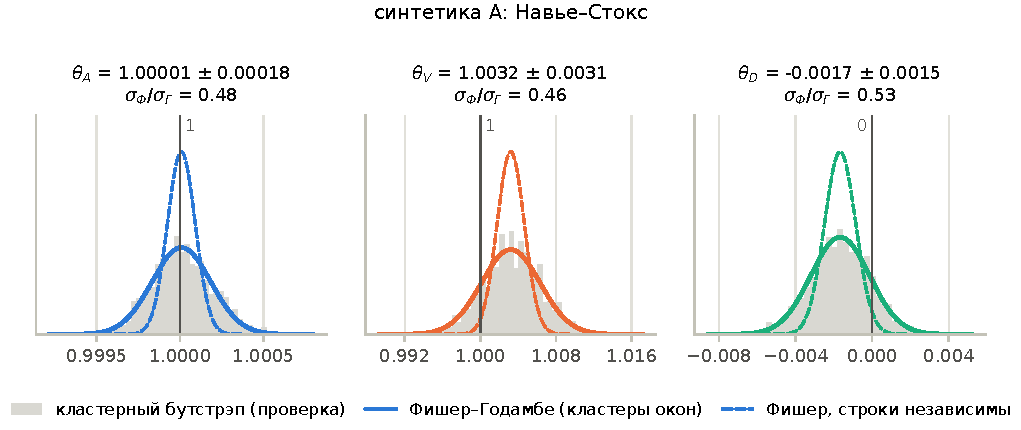
\includegraphics[width=\textwidth]{methods_syn_a}
  \par\medskip\raggedright\small
  \textbf{Сравниваем} две оценки метода 1.4 — Годамбе и наивного Фишера — и бутстрэп как проверку.
  Бутстрэп совпадает с Годамбе; наивный Фишер уже в \NarrowSynMin–\NarrowSynMax{} раза: перекрывающиеся окна
  не независимы.
  Оценки несмещены (истина 1, 1, 0).
\end{frame}

\begin{frame}{5. Синтетика А: P против Q и решение}
  \centering
  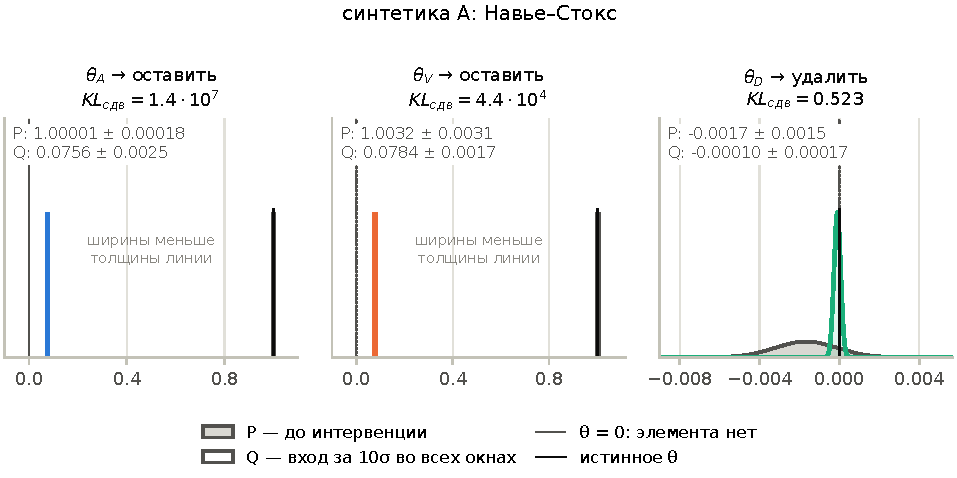
\includegraphics[width=\textwidth]{pq_syn_a}
  \par\smallskip\raggedright\footnotesize
  \textbf{Сравниваем:} $P$ — параметр на данных; $Q$ — после выноса входа элемента за $10\sigma$ во всех окнах.
  \begin{itemize}
    \item $A$, $V$: центр $Q$ уходит к нулю, $\KLs\gg\Threshold$ $\Rightarrow$ \textcolor{keep}{\textbf{оставить}} — верно.
    \item $D$: сдвиг — шум, $\KLs=\SynAKLD<\Threshold$ $\Rightarrow$ \textcolor{drop}{\textbf{удалить}} — верно.
  \end{itemize}
\end{frame}

\begin{frame}{5. Синтетика Б: расстояние от гиперпараметров $k$ и $q$}
  \centering
  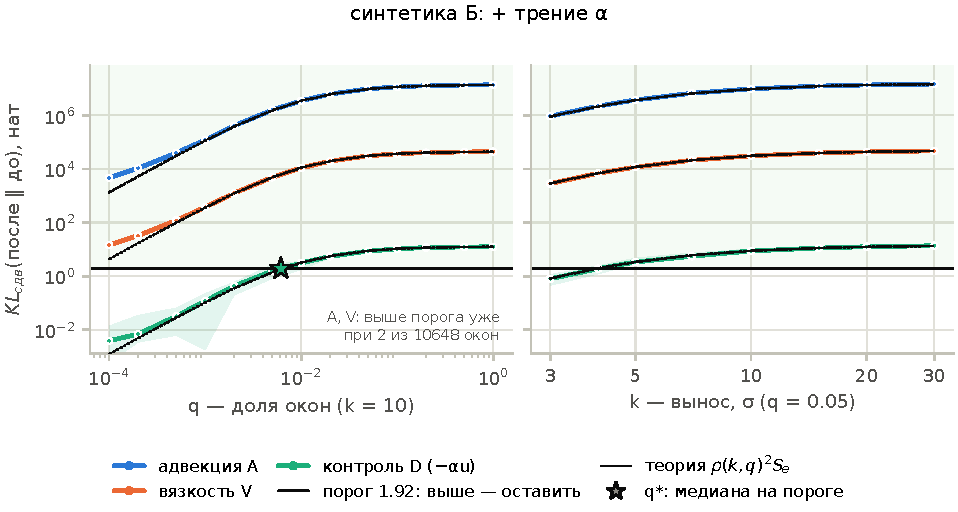
\includegraphics[width=\textwidth]{kl_syn_b}
  \par\smallskip\raggedright\footnotesize
  Трение есть: $\hat\alpha=\SynBThetaD$ (истина 0.01), $\KLs=\SynBKLD$ $\Rightarrow$ \textcolor{keep}{\textbf{оставить}}.
  Звезда — $q^*$: слабый элемент заметен при \SynBQstarD{} испорченных окон, $A$ и $V$ — уже при 2 окнах.
  На синтетике А $D$ ниже порога при любых $k$, $q$.
\end{frame}

\begin{frame}{5. Проверка ширины: \MCcount{} реализаций DNS}
  \centering
  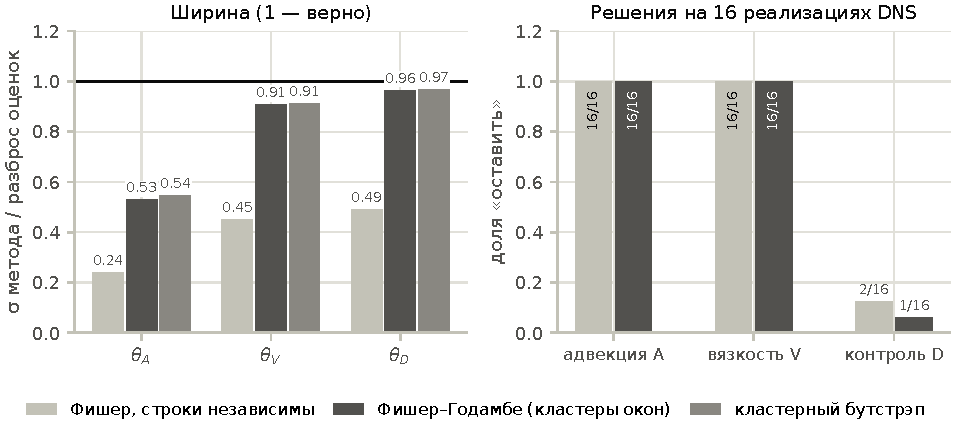
\includegraphics[width=\textwidth]{monte_carlo}
  \par\smallskip\raggedright\small
  \begin{itemize}
    \item Наивный Фишер занижает ширину в \MCFisherUnderMin–\MCFisherUnderMax{} раза $\Rightarrow$ чаще оставляет
      несуществующий $D$ (\MCFisherD{} против \MCGodambeD{}; теория: \MCFisherDExpected{} и \MCGodambeDExpected{} из \MCcount).
    \item Годамбе верен для $V$, $D$; для $A$ занижен в \MCGodambeUnderA{} раза — на решение не влияет ($S_A\sim10^7$).
  \end{itemize}
\end{frame}

% ---------- реальные ----------
\begin{frame}{6. Эксперимент: распределения по методам}
  \centering
  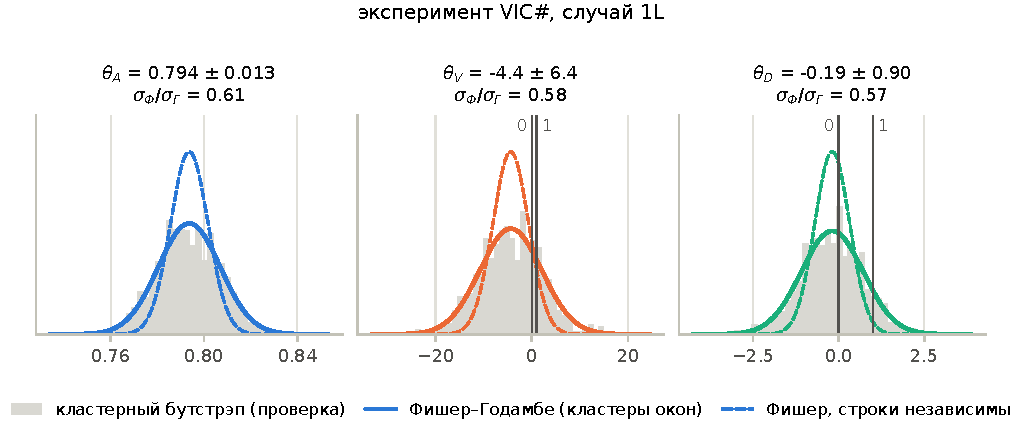
\includegraphics[width=\textwidth]{methods_real}
  \par\smallskip\raggedright\footnotesize
  \begin{itemize}
    \item $\theta_A=\RealThetaA$: адвекция видна; меньше 1 — шум и сглаживание входа.
    \item $\theta_V=\RealThetaV$: значение ЛР~1 ($\theta_V=1$) в \VinSigma$\sigma$ от нуля — вязкость не видна;
      в ЛР~1 подгонка $\nu$ упёрлась в границу поиска.
    \item Фишер уже Годамбе в \NarrowRealMin–\NarrowRealMax{} раза; бутстрэп совпадает с Годамбе.
  \end{itemize}
\end{frame}

\begin{frame}{6. Функция ошибки: L2 и Хьюбер}
  \centering
  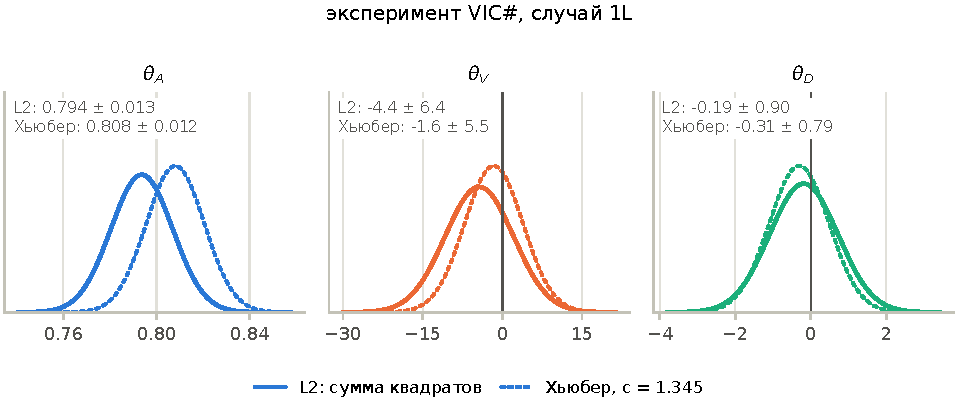
\includegraphics[width=\textwidth]{losses_real}
  \par\medskip\raggedright\small
  Хьюбер ослабляет хвосты остатков: $\theta_A$ сдвигается на \HuberShiftA$\sigma$, $\theta_V$ и $\theta_D$ остаются
  в пределах $\sigma$ от нуля. \textbf{Решение не меняется}: все 4 сочетания
  (функция ошибки $\times$ оценка информации) согласны для всех элементов.
\end{frame}

\begin{frame}{6. Эксперимент: P против Q и решение}
  \centering
  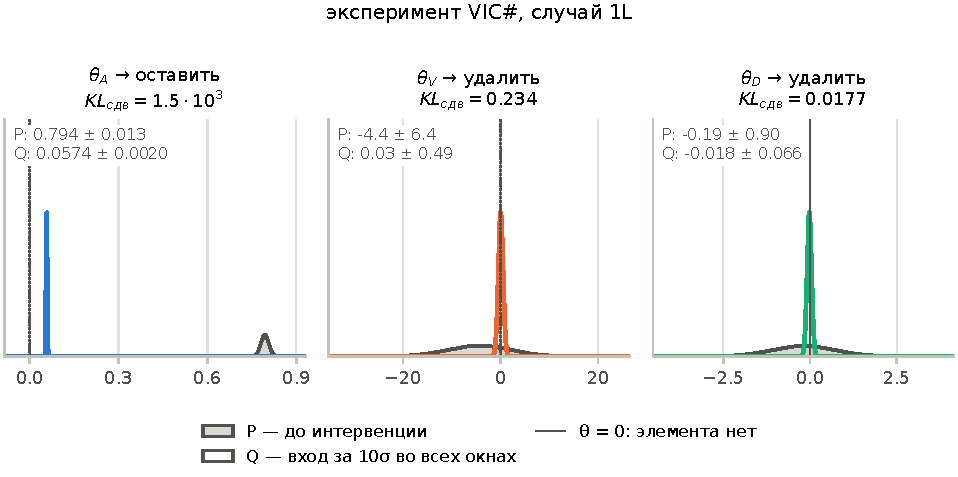
\includegraphics[width=\textwidth]{pq_real}
  \par\smallskip\raggedright\small
  \begin{itemize}
    \item $A$: $\KLs=\RealKLA$ $\Rightarrow$ \textcolor{keep}{\textbf{оставить}}.
    \item $V$, $D$: $Q$ сузилось, но центр сдвинулся меньше чем на $1\sigma$: $\KLs=\RealKLV$ и $\RealKLD$
      $\Rightarrow$ \textcolor{drop}{\textbf{удалить}}.
  \end{itemize}
\end{frame}

\begin{frame}{6. Расстояние от гиперпараметров $k$ и $q$}
  \centering
  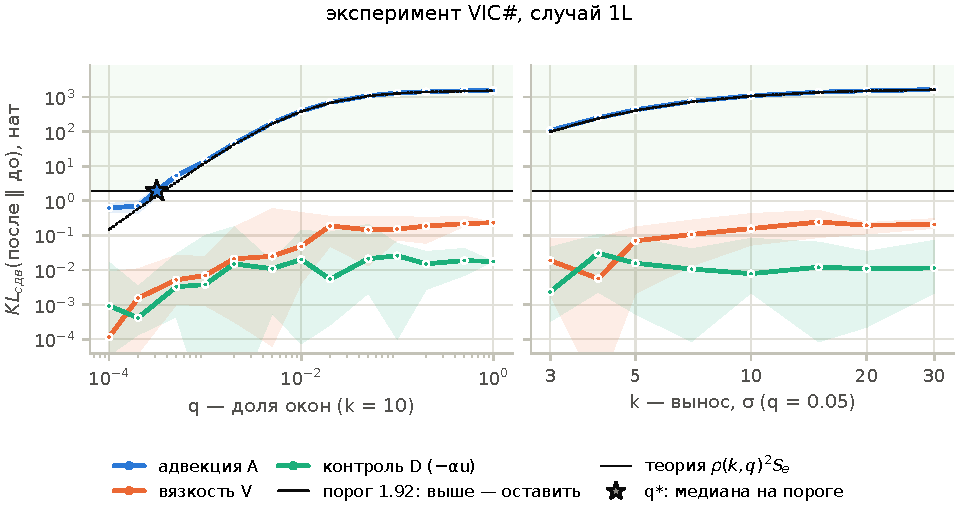
\includegraphics[width=\textwidth]{kl_real}
  \par\smallskip\raggedright\footnotesize
  $A$ пересекает порог при $q^*=\RealQstar$ (\RealQstarWindows{} окна из \RealWindows).
  $V$ и $D$ ниже порога при любых $k$ и $q$: сдвиг растёт, но не выше \RealPlateauV{} и \RealPlateauD{} —
  центр уходит самое большее в ноль, а ноль ближе $\sigma$ к оценке.
  Теория $\rho^2S_A$ верна при $q\gtrsim5\cdot10^{-4}$.
\end{frame}

\begin{frame}{6. Почему в правиле только сдвиг}
  \centering
  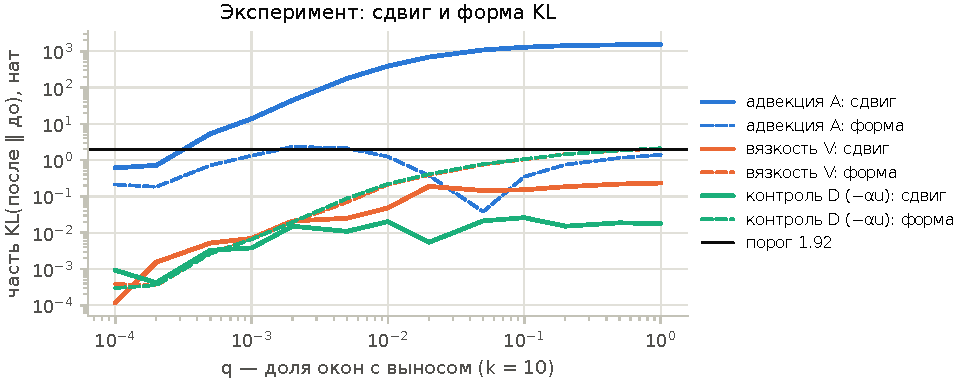
\includegraphics[width=\textwidth,height=0.55\textheight,keepaspectratio]{kl_parts_real}
  \par\medskip\raggedright\small
  Форма (штрих) растёт у всех элементов одинаково; у несуществующих $V$ и $D$ при $q=1$ она выше порога
  (\RealShapeV{} и \RealShapeD{} нат). Полный KL «оставил» бы всё: он реагирует на сам факт интервенции.
  Сдвиг разделяет $A$ и $V$ на \OrdersAV{} порядка.
\end{frame}

\begin{frame}{6. Чувствительность: функция ошибки и вид интервенции}
  \centering
  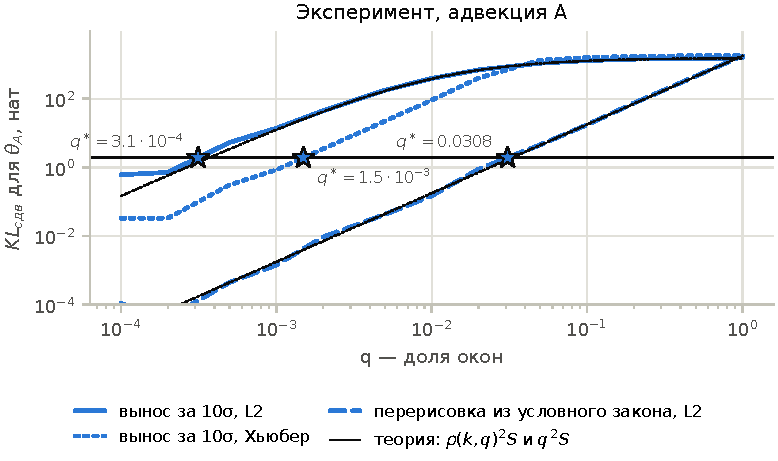
\includegraphics[width=0.9\textwidth,height=0.58\textheight,keepaspectratio]{q_sensitivity_real}
  \par\smallskip\raggedright\small
  \begin{itemize}
    \item Хьюбер гасит первые выбросы: $q^*$ в \HuberRatio{} раз больше, при $q\gtrsim5\,\%$ кривые сходятся.
    \item Перерисовка из условного закона (плацебо [9]) теряет информацию линейно, $\rho=q$: $q^*$ в
      \PlaceboRatio{} раз больше. Выброс за $10\sigma$ действует через вес $k^2$.
  \end{itemize}
\end{frame}

\begin{frame}{6. Вариант: вынос значений листьев на сетке}
  \centering
  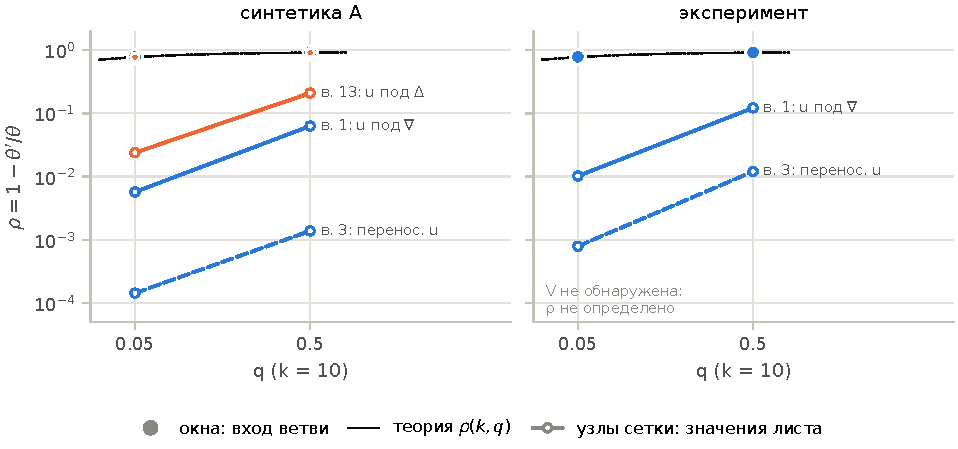
\includegraphics[width=\textwidth]{leaf}
  \par\smallskip\raggedright\footnotesize
  Значения $u$ в вершинах 1, 3, 13 выносятся за $10\sigma$ условного закона по шести соседям
  (гауссово марковское поле [10]).
  Поле гладкое: условная $\sigma\approx$ \GridSigmaReal{} маргинальной, слабая форма усредняет выбросы —
  параметр теряет в \LeafLossMin–\LeafLossMax{} раз меньше. При $q=5\,\%$ адвекция была бы не видна
  ($\KLs=\LeafKL$ против \WindowKL{} для окон) $\Rightarrow$ основная интервенция — на входы окон.
\end{frame}

\begin{frame}{6. Устойчивость к размеру пробных окон}
  \centering
  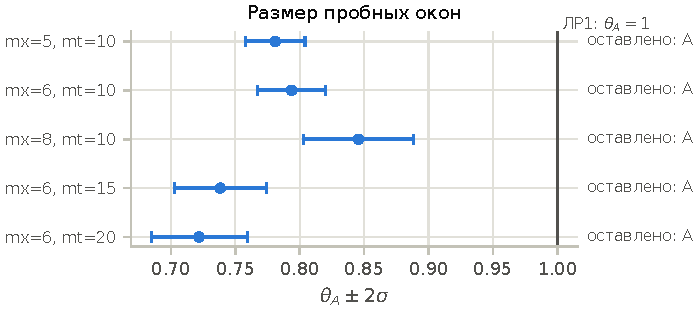
\includegraphics[width=0.85\textwidth,height=0.5\textheight,keepaspectratio]{scales}
  \par\medskip\raggedright\small
  Пять размеров окон — решение одно: остаётся только адвекция. $\theta_A$ меняется от \ThetaAmin{} до \ThetaAmax:
  коэффициент эффективный, он зависит от масштабов, которые усредняет окно (шум и сглаживание входа),
  а не от структуры модели.
\end{frame}

\begin{frame}{6. Итог по эксперименту: обратное исключение}
  \scriptsize
  Для каждого элемента: вход за $10\sigma$ во всех окнах, распределение до ($P$) и после ($Q$), сдвиговая часть KL.
  \medskip

  \centering
  \setlength{\tabcolsep}{3pt}
  \begin{tabular}{@{}lcccc>{\raggedright\arraybackslash}p{3.3cm}@{}}
    \toprule
    элемент & $P$ & $Q$ & $\KLs$ & форма & решение и почему \\
    \midrule
    адвекция $A$ & $\RealThetaA$ & $\RealQA$ & $\RealKLA$ & $\RealShapeA$ & \textcolor{keep}{\textbf{оставить}}: $\KLs\gg\Threshold$ \\[0.3em]
    вязкость $V$ & $\RealThetaV$ & $\RealQV$ & $\RealKLV$ & $\RealShapeV$ & \textcolor{drop}{\textbf{удалить}}: сдвиг $<1\sigma$ \\[0.3em]
    контроль $D$ & $\RealThetaD$ & $\RealQD$ & $\RealKLD$ & $\RealShapeD$ & \textcolor{drop}{\textbf{удалить}}: сдвиг $<1\sigma$ \\
    \bottomrule
  \end{tabular}
  \par\medskip\raggedright
  \textbf{Порядок:} шаг 1 — полная модель, удаляем слабейший $D$; шаг 2 — переоценка, $V$: $\KLs=\StepKLV$
  $\Rightarrow$ удаляем; шаг 3 — остаётся $A$. $R^2$: \RsqFull{} $\to$ \RsqFinal{} — $V$ и $D$ ничего не объясняют.
  Все 4 сочетания (L2/Хьюбер $\times$ Фишер/Годамбе) согласны на каждом шаге.
\end{frame}

% ---------- что удаляется ----------
\begin{frame}{7. Что удаляется: граф}
  \centering
  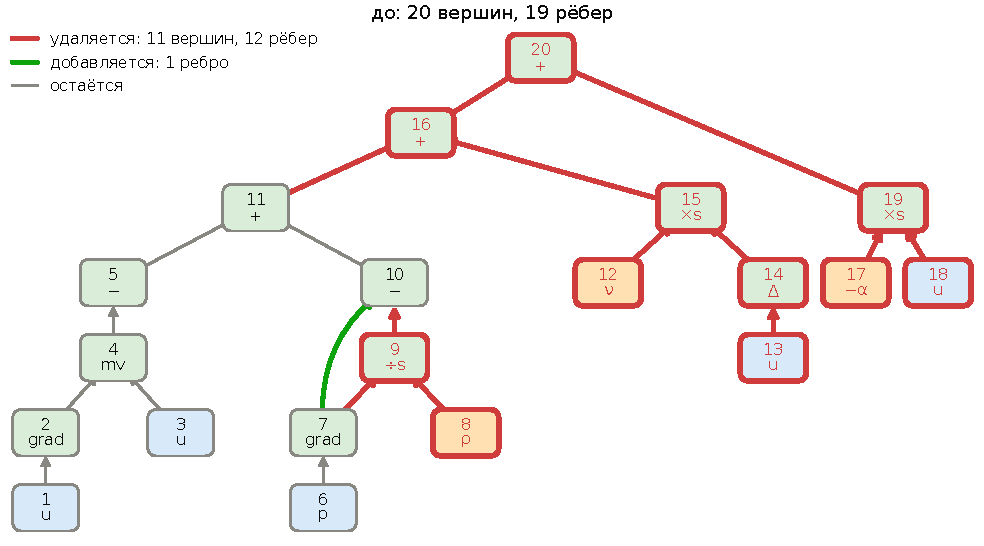
\includegraphics[width=\textwidth,height=0.64\textheight,keepaspectratio]{decision_real}
  \par\medskip\raggedright\small
  \textcolor{drop}{\textbf{Красное}} — удаляются $\rho$ и деление (8, 9: $\rho$ сливается в $P=p/\rho$), ветвь вязкости
  (12–16) и кандидат (17–20); \textcolor{keep}{\textbf{зелёное}} — новое ребро 7$\to$10.
\end{frame}

\begin{frame}{7. Граф и матрица связей после удаления}
  \begin{columns}[c]
    \begin{column}{0.44\textwidth}
      \centering
      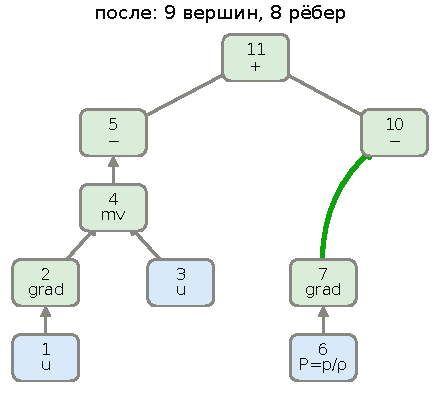
\includegraphics[width=\linewidth]{after_real}
    \end{column}
    \begin{column}{0.55\textwidth}
      \centering
      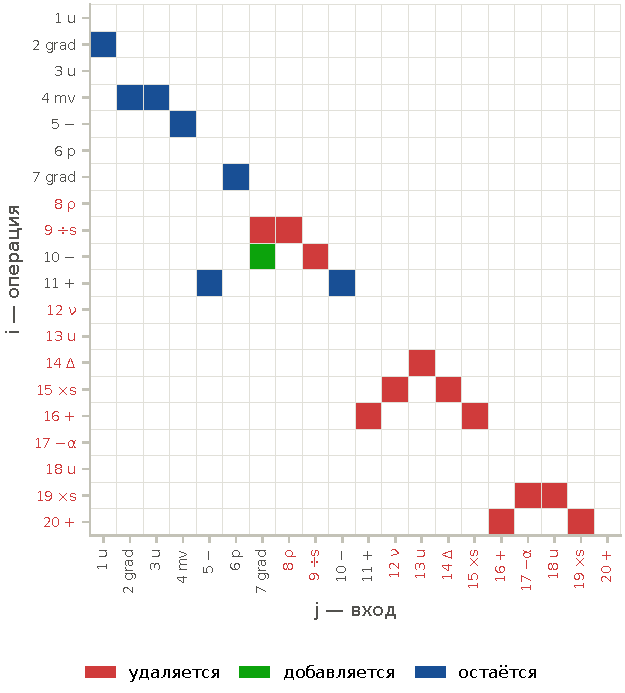
\includegraphics[width=\linewidth,height=0.68\textheight,keepaspectratio]{adjacency_real}
    \end{column}
  \end{columns}
  \par\smallskip\small
  Было \GraphBeforeText, стало \GraphAfterRealText:
  уравнение Эйлера с кинематическим давлением. $Z[i,j]=1$ — вершина $j$ на входе вершины $i$.
\end{frame}

\begin{frame}{8. Решение}
  \small
  \begin{tabular}{@{}lcccc@{}}
    \toprule
    данные & $A$ & $V$ & $D$ & вершин / рёбер \\
    \midrule
\DecisionRows
    \bottomrule
  \end{tabular}
  \medskip

  Итоговая модель для эксперимента:
  \[
    \partial_t u=-\theta_A(\nabla u)\,u-\nabla P,\qquad\nabla\cdot u=0 .
  \]
  \footnotesize
  \begin{itemize}
    \item На синтетике критерий восстанавливает истинную структуру, включая слабое трение.
    \item На эксперименте вязкость при разрешении 1.6 мм не видна, $p$ и $\rho$ — только как $P=p/\rho$.
    \item Решение не зависит от функции ошибки, оценки информации и размера окон.
    \item Ширина решает: наивная матрица Фишера занижает её в \MCFisherUnderMin–\MCFisherUnderMax{} раза.
  \end{itemize}
\end{frame}

% ---------- источники ----------
\begin{frame}{Источники}
  \tiny
  \begin{enumerate}
    \setlength{\itemsep}{0.1em}
    \item[{[1]}] Hillestad et al. Wake of a model wind turbine: volumetric velocity measurements. \emph{Phys.\ Rev.\ Fluids} 11, 014701 (2026); DataverseNO doi:10.18710/SX0ZQT
    \item[{[2]}] А.~Эйнуллаев. ЛР~1: github.com/Chessmatus/navie-stocks-aero, коммит 13e4e8f
    \item[{[3]}] D. J. C. MacKay. A practical Bayesian framework for backpropagation networks. \emph{Neural Comput.} 4, 448–472 (1992)
    \item[{[4]}] М. П. Кузнецов, А. А. Токмакова, В. В. Стрижов. Анализ выбора моделей и оценка гиперпараметров. \emph{Информатика и её применения} (2016)
    \item[{[5]}] V. P. Godambe. An optimum property of regular maximum likelihood estimation. \emph{Ann.\ Math.\ Statist.} 31, 1208–1211 (1960)
    \item[{[6]}] K.-Y. Liang, S. L. Zeger. Longitudinal data analysis using generalized linear models. \emph{Biometrika} 73, 13–22 (1986)
    \item[{[7]}] P. J. Huber. Robust estimation of a location parameter. \emph{Ann.\ Math.\ Statist.} 35, 73–101 (1964)
    \item[{[8]}] F. Pukelsheim. The three sigma rule. \emph{Amer.\ Statist.} 48(2), 88–91 (1994)
    \item[{[9]}] E. Candès et al. Panning for gold: model-X knockoffs. \emph{JRSS B} 80, 551–577 (2018)
    \item[{[10]}] H. Rue, L. Held. \emph{Gaussian Markov Random Fields.} Chapman \& Hall (2005)
    \item[{[11]}] R. Frisch, F. V. Waugh. \emph{Econometrica} 1, 387–401 (1933); M. C. Lovell. \emph{JASA} 58, 993–1010 (1963)
    \item[{[12]}] S. Kullback, R. A. Leibler. On information and sufficiency. \emph{Ann.\ Math.\ Statist.} 22, 79–86 (1951)
    \item[{[13]}] S. Amari. \emph{Information Geometry and Its Applications.} Springer (2016)
    \item[{[14]}] B. Hassibi, D. G. Stork. Second order derivatives for network pruning: Optimal Brain Surgeon. \emph{NIPS} 5 (1993)
    \item[{[15]}] D. A. Messenger, D. M. Bortz. Weak SINDy for partial differential equations. \emph{J.\ Comput.\ Phys.} 443, 110525 (2021)
  \end{enumerate}
\end{frame}

\end{document}
